 % Don't report over-full \bv-boxes if over-edge is small
% topmargin is 1/2 inch (note negative value)
% left margin is 1 inch on right-hand pages
% same for left-hand pages in \AtBeginDocument
% leaves 1 inch for the right margin
% 9 inches reserved for the text.
% THEOREM Environments ---------------------------------------------------
% MATH -------------------------------------------------------------------
%\DeclareMathOperator{\RE}{Re}
%\DeclareMathOperator{\IM}{Im}
%\DeclareMathOperator{\ess}{ess}
%\newcommand{\X}{\mathcal{\bfX}}
%% Maxims' commands
%\newcommand{\bu} {\mathbf{u}}
%\newcommand{\bv} {\mathbf{v}}
%\def\cdt{{\hskip-0.08ex\cdot\hskip-0.08ex}}
%%% ----------------------------------------------------------------------

\documentclass[12pt]{article}%
\usepackage{amsmath}
\usepackage{amssymb}
\usepackage{amsbsy}
\usepackage{amsthm}
\usepackage{epsfig}
\usepackage{wrapfig}
\usepackage{color,cancel}
\usepackage{fullpage}
\usepackage{float}
\usepackage{ulem}
\usepackage{setspace}
\usepackage{caption}
\usepackage{subcaption}

\DeclareMathOperator{\diam}{diam}
\newcommand{\vecb}[1]{\mathbf{#1}}

\vfuzz2pt
%\topmargin=-.5in
%\oddsidemargin=0.5in
%\evensidemargin=0.5in
%\textwidth=6.in
%\textheight=9.1in

\bibliographystyle{acm}

\date{}

\title{Image Segmentation}


\author{
 Nathan D. Heavner
      \and
  Rachel Tutmaher
  	\and
	James Folberth
}

\begin{document}


\maketitle

\section{Results}

In this section, we demonstrate the efficacy of the segmentation algorithm. We first demonstrate in Figure~\ref{fig:disk} the improvement in segmentation accuracy obtained by taking multilevel intensity variance into account. The image in Figure~\ref{fig:disk} contains two segments which have different textures (variance within the segment) but identical average intensities. When we do not take multilevel variance into account, the algorithm detects only one segment. When we rescale the weighting matrix using the variance of each block, however, the two segments are successfully detected.

\begin{figure}
\centering

\includegraphics[width=0.2\textwidth,height=0.2\textwidth]{checker_disk_good_seg_1.png} \hspace{.45cm}

\includegraphics[width=0.2\textwidth,height=0.2\textwidth]{checker_disk_good_seg_2.png}
\caption{Without taking multilevel variance into account, the algorithm detected only one segment (the entire image). Rescaling the weighted graph using multilevel variance results in the segmentation shown above. Parameters used: $n = 60$, $\alpha = 10$, $\tilde{\alpha} = 10$, $\beta = 10$, $\theta = 0.1$, $\gamma = 0.1$, $d_1 = 0.15$, $\sigma = 5$, $\rho = 1$.}
\label{fig:disk}
\end{figure}

Next, we demonstrate the effect of making the saliency measure invariant of the segment scale by normalizing the similarity-weighted boundary length and area. With the usual saliency measure, it is much harder for the algorithm to detect the segments because the boundary length is much greater than the segment area compared to a simpler shape such as a circle. With the author's proposed scale invariant measure, the segment is easily detected.

\begin{figure}

\begin{subfigure}[b]{\textwidth}
\centering

\includegraphics[width=0.2\textwidth,height=0.2\textwidth]{spiral_bad_seg_1.png} \hspace{.45cm}

\includegraphics[width=0.2\textwidth,height=0.2\textwidth]{spiral_bad_seg_2.png} \hspace{.45cm}

\includegraphics[width=0.2\textwidth,height=0.2\textwidth]{spiral_bad_seg_3.png}
\subcaption{Segmentation without scale invariant saliency measure.}
\end{subfigure}

\vspace{.45cm}

\begin{subfigure}[b]{\textwidth}
\centering

\includegraphics[width=0.2\textwidth,height=0.2\textwidth]{spiral_good_seg_1.png} \hspace{.45cm}

\includegraphics[width=0.2\textwidth,height=0.2\textwidth]{spiral_good_seg_2.png}
\subcaption{Segmentation with scale invariant saliency measure.}
\end{subfigure}

\caption{Parameters used: $n = 64$, $\alpha = 10$, $\tilde{\alpha} = 10$, $\beta = 10$, $\theta = 0.09$, $\gamma = 0.08$, $d_1 = 0.15$, $\sigma = 7$, $\rho = 1$.}
\label{fig:spiral}

\end{figure}

The remaining figures demonstrate the performance of the algorithm with more complex images. The performance is quite good. In the cases where the segmentation is ``incorrect," we can reasonably attribute this to human intelligence rather than algorithm performance. In Figure~\ref{fig:peppers}, for example, one segment includes the fruit from one pepper and the stem from another. From a purely visual perspective, these segments look very reasonable. It's only because humans know that the stem and fruit go together, and must be arranged in a particular orientation, that we would segment the image differently from the algorithm.

\begin{figure}
\centering
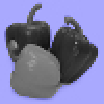
\includegraphics[width=0.2\textwidth,height=0.2\textwidth]{peppers_seg_1.png} \hspace{.45cm}
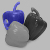
\includegraphics[width=0.2\textwidth,height=0.2\textwidth]{peppers_seg_2.png} \hspace{.45cm}

\includegraphics[width=0.2\textwidth,height=0.2\textwidth]{peppers_seg_3.png} \\ \vspace{.45cm}
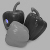
\includegraphics[width=0.2\textwidth,height=0.2\textwidth]{peppers_seg_4.png} \hspace{.45cm}

\includegraphics[width=0.2\textwidth,height=0.2\textwidth]{peppers_seg_5.png}
\caption{Parameters used: $n = 50$, $\alpha = 50$, $\tilde{\alpha} = 4$, $\beta = 10$, $\theta = 0.1$, $\gamma = 0.15$, $d_1 = 0.15$, $\sigma = 5$, $\rho = 1$.}
\label{fig:peppers}
\end{figure}

One weakness of the algorithm, mentioned by the authors, is the large number of parameters and difficulty in choosing them correctly. Currently, parameters are chosen by guessing and checking, which obviously presents a large obstacle to the algorithm's robustness and usefulness in industrial applications. There are, however, some general guidelines that can be used to improve the segmentation accuracy.

\begin{enumerate}

\item If the image has low contrast levels, increase the first-level intensity scaling factor $\alpha$. This amplifies the difference in intensity between two nodes in the weighted graph matrix.

\item If the image segments are likely to be bordered by very dark or bright regions (as is the case with bright field microscopy cell images), there is a chance that these borders will become salient segments themselves. To avoid this, decrease the coarse-level rescaling factor $\tilde{\alpha}$, since a large $\tilde{\alpha}$ causes nodes with high average intensity to become more disconnected from their neighbors.

\item If the algorithm detects too many segments, then several parameter changes may be beneficial. Decreasing $\theta$ yields stronger connections between nodes; decreasing $\gamma$ provides a stricter salience threshold; and increasing $\sigma$ prevents segment detection on fine levels. All these changes make it more difficult for nodes to be salient and result in fewer segments.

\end{enumerate}


\end{document}

%%% Local Variables: 
%%% mode: latex
%%% TeX-master: t
%%% End: 
